\begin{frame}{Sicherheitslücken in der Logik}
  \begin{quote}
    \normalsize
    By causing a failure condition in the 2.4 GHz radio frequency band,
    the security system \textbf{does not fail closed} with an assumption that an
    attack is underway. Instead, \textbf{the system fails open}, and the security
    system continues to report that "\alert{All sensors are in-tact and all doors
    are closed. No motion is detected.}"
    \begin{flushright}
      \small
      -- Rapid7 (05.01.2016), \href{https://community.rapid7.com/community/infosec/blog/2016/01/05/r7-2015-23-comcast-xfinity-home-security-system-insecure-fail-open}{R7-2015-23}
    \end{flushright}
  \end{quote}
\end{frame}

\begin{frame}{Sicherheitslücken im Protokoll}
  \begin{quote}
    \normalsize
    \textbf{Verschlüsselung als Satire}\\
    Grundsätzlich kommunizieren die Geräte verschlüsselt.
    Jedoch schreibt das ZigBee-Konsortium vor, dass alle Geräte
    \alert{ein und dasselbe Schlüsselpaar} (Fallback Key) kennen
    und akzeptieren müssen – und dieses asymmetrische Schlüsselpaar ist
    \alert{öffentlich bekannt}.
    \begin{flushright}
      \small
      -- \url{http://heise.de/-3010287}
    \end{flushright}
  \end{quote}
\end{frame}

\begin{frame}{}
  \begin{center}
    \makebox[\textwidth][c]{
\includegraphics[width=1\paperwidth]{images/zigbee}}

    \url{http://www.zigbee.org}
  \end{center}
\end{frame}

\begin{frame}{}
  \begin{center}
    \vspace{-0.2cm}
    \makebox[\textwidth][c]{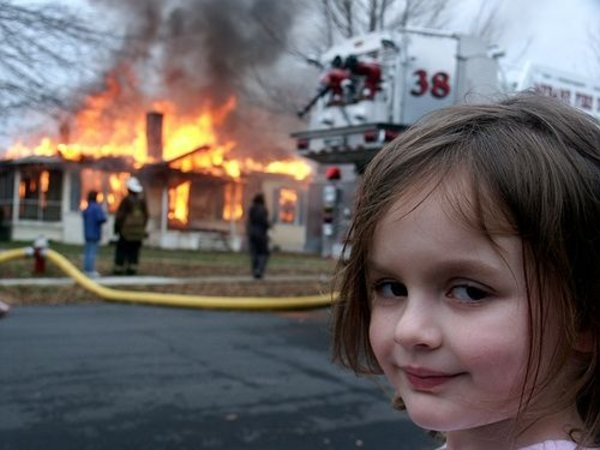
\includegraphics[width=1\paperwidth]{images/desastergirl}}
    \label{fig:disaster}
  \end{center}
\end{frame}
